\documentclass{article}
\usepackage[utf8]{inputenc}
\usepackage{enumitem}
\usepackage{graphicx}
\usepackage{color}
\usepackage{rotating}
\usepackage{adjustbox}
\usepackage{multirow} 

\title{Next Generation User Interface: \\Redefining file browsing}
\author{
  De Bleser, Jonas\\
  \texttt{jdeblese@vub.ac.be}\\
  Rollnumber: 0508848
  \and
  Carraggi, Nicolas\\
  \texttt{ncarragg@vub.ac.be}\\
  Rollnumber: 0093262
  \and
  Spruyt, Valentijn\\
  \texttt{vspruyt@vub.ac.be}\\
  Rollnumber: 0508466
}
\date{\today}

\begin{document}

\maketitle

\tableofcontents

\section{Problem statement}
The current state of file browsing is very similar on most desktop platforms. Based on an observation of the current file browsers, we conclude that each file browser consists of two important parts: a tree view and a content view. The first view shows the hierarchy and structure of the file system, whereas the second view simply shows the contents of one level in the hierarchy.  We also note that browsing through these views is solely based on mouse and keyboard input. These observations exists for quite a long time and have not changed in the past decades. Therefore, our goal is to redefine file browsing by means of hand gestures, a flat file hierarchy and a more simple, intuitive interface. In the end, we are not really trying to solve a problem, but we rather want to create another approach towards file browsing.

Our approach consists of groups and tags to create a flat, nevertheless usable, hierarchy of files. A group is a general representation of a cluster of files. A tag is similar to a label and represents a keyword (e.g. \textit{vacation}, \textit{Belgium}, \textit{cat}). A group is created by assigning it a name and several tags. Those tags determine which files will be related to this group. Assuming we add the tags \textit{vacation} and \textit{Belgium} to a group, it will cluster all files that have one of the aforementioned tags into that group. We decided to not support the feature of nested groups, because we want a clear overview of all groups. Nevertheless, some sort of nesting can also be achieved using our system. In terms of customizability, groups and tags can also have a color to characterize the appearance. Our idea was to utilize the gestures of the Myo to speed up the overall flow of managing a file system. Actions like cut, delete, etc would be mapped to a single gesture, reducing the amount of clicks from two (i.e. open context menu, click menu option) to one (i.e. simply do a gesture). Shortcut keys are, of course, another way to reduce the amount of clicks. Although, this still requires clicking the file, whereas with the Myo we simply hover to select. Unfortunately, this didn't go as expected as we explain in \ref{sec:challenges}.

\section{Requirements analysis}

\subsection{Usability requirements}

\subsection{Functional Requirements}
TODO: alles naar tabel NICOHHHHHHHHHHHHH
The two main functionalities of our program consist of browsing and manipulating files, as well as providing a way of structuring folders in a custom way. The user should be able to browse the files easily using intuitive gestures. Next to browsing, we will introduce a new way of structuring files and folders, customized to the user its preferences. What follows next is a more specified way on how the file browsing will (probably) work. 
\\\\
Selecting files and folders will be based on the direction we point with our arm. Hovering a certain folder will result in a (possibly customizable) preview. Browsing through the contents (i.e. files/folders) of a folder will be possible by rotating the arm and/or by doing the left and right swipe gesture to move backward and forward through the list of contents. To rename and search files we will use the keyboard as the primary input device, but we will also attempt to use voice recognition software as a supplementary input source to support people with a physical disability.
\\\\
As far as customization of folders goes, we will attempt to make a more user-friendly way of grouping together files and folders, possibly using some sort of tagging system. In this way content specific folders are created and they will also have the ability to specify a custom view of the content. The concept of customization is still vague because we haven't decided yet on how we are going to implement it.
\\\\
Manipulating the file system is done by performing an arm gesture, after which a menu similar to the one in figure 1. This menu will consist of the possible actions that can be executed on the selected file(s) and/or folder(s).
\\\\
Navigation through the folder hierarchy is done by implementing some sort of breadcrumbs. Our initial thought was to use the  up- and downward gesture in order to go up and down respectively in our tree of folders.

\begin{center}
    \begin{tabular}{ | l | l | p{5cm} |}
    \hline
    Type & Requirement & Motivation 
		\\ \hline
		
    \multirow{5}{*}{Functional Requirement} 
		& Browse through files \& folders & TODO
		\\ \cline{2-3}
		& Manipulating files with default actions & TODO
		\\ \cline{2-3}
		& Search through tagged files, groups and tags & TODO
		\\ \cline{2-3}		
		& Usage of menu & TODO
		\\ \cline{2-3}
		& Tag files & TODO
		\\ \cline{2-3}
		& Create groups & TODO
		\\ \cline{2-3}
		& NOGGGG NICOHH & TODO
		\\ \hline		
		
    \multirow{2}{*}{Data Requirement} & Access to file system & The data we want to display and manipulate in our user interface comes straight from the underlying file system, i.e. information about files and folders. Our application should be able to access the file system without limitation. 
		\\ \cline{2-3}
		& Store meta data & There has to be enough free storage space to store meta data of our application. This will be in the form of a database file which contains relations between groups, tags, etc.
		\\ \hline

    \multirow{2}{*}{Environmental Requirement} & Enough moving-space & The environment must allow a person to easily move the arm of the user in front of the screen.
			\\ \cline{2-3}
		& Cross-platform application & The user should not be limited to a specific operating system to use the application
    \end{tabular}
\end{center}

\section{Design and interactions}

Our approach to the interaction design is activity-centered design because we are focusing on the behavior of a file system. 

\subsection{Interactions}
Instructing interactions is done mainly by the Myo. We define the following five gestures: \texttt{FIST}, \texttt{FINGERS\_SPREAD}, \texttt{WAVE\_IN}, \texttt{WAVE\_OUT} and \texttt{DOUBLE\_TAP}. We decided not to use the \texttt{WAVE\_OUT} gesture because the Myo did not recognize this gesture very well. Also we noticed that, while performing the gesture, the position of the pointer drifted away quite far, thus doing the gesture on another position then originally intended. The \texttt{DOUBLE\_TAP} gesture is used to switch between the native mode and the group mode. Specifically for modals, we use \texttt{FIST} to accept and \texttt{WAVE\_IN} to cancel. To open a menu on a specific item (i.e. file, folder, group and tag) we use the \texttt{FIST} gesture, which shows extra options that are applicable to that item. The \texttt{FINGERS\_SPREAD} gesture on an item (and other interaction elements) performs the same operation as a normal click would do. Originally, we thought of using voice recognition to input text but it wasn't accurate enough to fulfill our requirements. As a result, all input interaction is done via keyboard. Another interaction we planned to do is drag and drop of files/folders to groups. However, we didn't manage to do this because of limited gestures of Myo. Interaction with the screen is not limited to a computer screen, since you can use any screen that is connected to your computer.

\subsection{Design}

Since files, groups and tags are the most important part of our application, we decided to place them on the top of our application for quick access. The search bar is also placed on top because this is a feature that is often used. An extra toolbar was added to the left to provide actions that target the whole view, but these are often create and edit actions. We followed the design of current file browsers to display files and folders, whereas for groups and tags we chose our own design.

We focused the design of our application on the abilities of the Myo. This includes large buttons, large icons, grid views instead of plain lists, a flat design without fancy things, etc. We introduced zooming of elements when the pointer hovers an item or a button in the menu. This gives a higher usability because of the small inaccuracy of the pointing. 

At first, we were going to use some sort of radial menu and the rotation of the Myo to select a option. However, we didn't manage to implement this for the Myo because the source code did not support adding custom events without rewriting it all. Therefore we opted to make a normal menu with options. We also think that the rotation gesture in combination of other gestures of the Myo is not accurate enough, so in the end we would have to switch to a normal menu anyways.

We tried to make sure we followed the most important principles such as consistency, feedback, simplicity and Gestalt principles.

\section{Technical report}

Our technical report includes the architecture and explains some challenges about the used frameworks and the Myo.
\subsection{Architecture}

We based our architecture on Java to support multiple platforms. We have tested our application on both Windows and Mac to make sure our application works correctly. Metadata for our application is stored using HSQLDB\footnote{http://hsqldb.org} (HyperSQL DataBase) using the schema shown in Figure \ref{dbmodel}. We also use Node.js\footnote{https://nodejs.org} as a web server to serve files to the front-end.  The user interface is build using HTML, CSS and JavaScript frameworks such as Bootstrap\footnote{http://getbootstrap.com}, Backbone.js\footnote{http://backbonejs.org}, Marionette.js\footnote{http://marionettejs.com} and Require.js\footnote{http://requirejs.org}. We made the decision to make the graphical user interface web-based, since it is a lot easier to customize the look and feel, as well as do advanced animations. To display the web content, we use JXBrowser which is a Java-based browser supporting Webkit\footnote{https://webkit.org}. Backbone.js is an MV* framework which provides us models, collections, views and additional functionalities to glue them together. However, it is very low level framework and therefore we use Marionette.js on top of it which gives us higher level components. For example, a \texttt{CollectionView} which provides us with all logic and functionalities to display a collection. In Backbone.js we would have to create such a common-used view from zero. We also use Require.js to work with dependencies for each file. In this way, only the required dependencies are fetched from the server, limiting the amount of requests to the server. However, once the application is finished, we can minify all dependencies to one file and simply load it using JxBrowser. As a result, we could remove the Node.js based web server entirely, but we left it for development purposes. Specifically, the only reason Node.js is used, is to avoid the same-origin policy problem with local dependencies. We also used a Java port\footnote{https://github.com/NicholasAStuart/myo-java} of the Myo SDK, instead of the default C/C++ SDK.

\begin{figure}[!ht]
  \centering
      \centerline{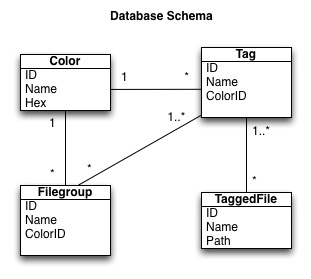
\includegraphics[width=0.5\textwidth]{Images/database.jpg}}
  \caption{The database schema}
	\label{dbmodel}
\end{figure}

\subsection{Challenges}
\label{sec:challenges}
In this section we will discuss some of the challenges we encountered during the development of our project.

\subsubsection{The Marionette.js framework}
One of the challenges of this project was the Marionette.js framework itself. Even though only one member of our team had experience with the framework, we all agreed on using it. The motivation for using this framework was that it has a neatly built model and view structure, which made it possible to write clean code that is fairly easy to read. The framework itself is a decent framework, but development went very slow because of the basic knowledge of JavaScript by the other two members. On the other side, by using this framework we increased our JavaScript skills, which will be handy for the future.

\subsubsection{Myo}
The Myo\footnote{https://www.myo.com/} bracelet is a something which can be used in a wide range of applications. When we watched a demo video, we immediately thought that it would be a nice thing to use for our project. The nice thing about the bracelet is that it already supports several basic gestures and that it can detect spatial arm movement, next to just gestures of the lower-arm. However, when we started the project, we thought of adding custom gestures which were detectable by the bracelet. We saw fairly soon that this wouldn't be optimal since it was already difficult enough for the bracelet to detect the basic gestures. This was a big issue for the development of our project. When we tried to test our application with gesture \texttt{X}, the chances were that the bracelet detected gesture \texttt{Y} instead, which lead to great frustration.
Another issue was the problem that comes with working with hardware, rather than software alone: Only one team member could take the Myo bracelet home and do some testing and programming with it. This caused delays in the development process, since it was very hard to synchronize work progress. An example: We decided to implement feature \texttt{A} in our application. One team member had set up the layout and views of the feature, another member coded some processing functions for the feature and the third team member was in charge of writing the code to send the myo gestures to our client side JavaScript. The problem was that, obviously, not everyone could work for the project 24/24 hours every day. This made development slower because we sometimes had to wait on another member to finish his assigned task. The other members couldn't just go and drive several tens of kilometers to go and fetch the Myo bracelet, so that they could write the code themselves.
A last issue was that the Myo bracelet needs some warming up and synchronization before you can use it. This synchronization phase requires the user to perform a \textit{wave-out} gesture for several seconds to even a minute long. This resulted into cramps in our lower arm more than once.

Finally, we had to find a good way to point precisely on the screen with the Myo. The data we get from the Myo are scaled x and y values. The x value ranges from 0 to scale, this range corresponds to one full body rotation with your arm stretched in front of you. The y value also ranges from 0 to scale, pointing to the floor will correspond to the value 0 and pointing to the ceiling will correspond to the max value. 

There are many ways of handling these x and y values to simulate the pointing to the screen. For the sake of simplicity we decided to let the user calibrate the screen at the start of the application. The user will have to follow the instructions on the screen. We ask the user to first point to the middle of the screen, make a fist gesture, then point to the left upper screen corner and finish with a fist gesture. Based on these two points we can determine the other three corners.  This is really simple, but yet very powerful because the user can decide how en where he will point, and it allows the user to point in a way he feels the most comfortable with.

For this project we assume that the user will calibrate the screen somewhere in front of him, so we will not handle the extreme cases where the user calibrates the screen pointing to the floor or to the ceiling. This is to avoid the 0 and max value, this also means the conversion of the y value of the Myo to the y value on the screen is straightforward. So the only real difficulty was converting the x value of the Myo to the x value on the screen. More specifically when the user calibrates the screen around the edge x values of the Myo. If the user calibrates the screen between the 0 and max value the conversion is straightforward. We will demonstrate and explain both cases.

Figure \ref{easyconv} demonstrates the easy case. We can see that the screen is inside the total range of x, thus the left-corner x value is greater than the center x value which is greater than the x value of the right-corner ( x2 $>$ x1 $>$ x3 ).


\begin{figure}[!ht]
  \centering
      \centerline{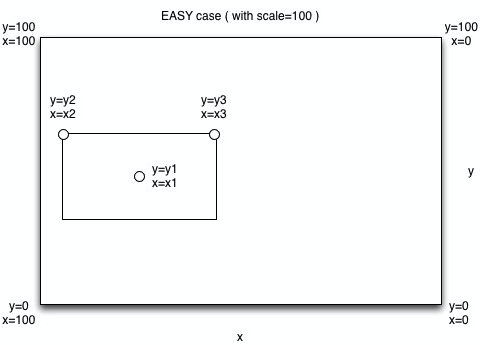
\includegraphics[width=1\textwidth]{Images/easy-conversion.png}}
  \caption{The easy conversion}
	\label{easyconv}
\end{figure}

In the difficult case on Figure \ref{diffconv}, the screen crosses the edge of the x range. The left-corner x value is smaller than the center x value ( x2 $<$ x1 ). This means the conversion of the x value was more complex.

\begin{figure}[!ht]
  \centering
      \centerline{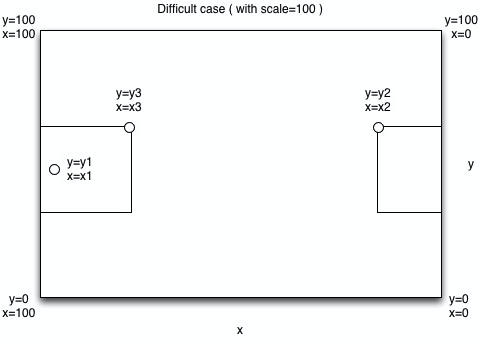
\includegraphics[width=1\textwidth]{Images/diff-conversion.png}}
  \caption{The difficult conversion}
	\label{diffconv}
\end{figure}


\subsubsection{JxBrowser}
To bridge the gap between Java and JavaScript, we used the JxBrowser component. When we initially looked the component up, it looked very promising. A 30-day trial was available so we could start right away. After that we could get a free educational license, after filling in some forms. We soon realized that the JxBrowser component was rather processor-heavy, and that its responsiveness was sometimes rather low. The component came in the form of a \textit{.jar} file, and modified something in the registry of our computer, so that we couldn't just use a new 30-day trial when the old one expired. This lead to several problems. In order to obtain an educational license, we first had to fill in a form with some information about the VUB. After that, we also had to ask Dr. Signer to send a recommendation mail to confirm that we are indeed students at the VUB. When the developers of the JxBrowser component finally sent us the license, it didn't work. There was some sort of bug that didn't change the registry key, so we kept getting the error that our 30-day trial had expired. By the time that we figured this out together with the developers, we had lost quite some time.
Our initial motivation to use a web based user interface, was the ease to create animations. However, towards the end, we noticed that those animations were not that smooth as expected. We think that this is the result of the single threaded nature of JavaScript and the continuously sending of Myo events to the web browser.

\subsection{Known bugs/incomplete logic}
\begin{itemize}
\item When navigating not all states are pushed to the history stack. This causes to go back to a different view when the back gesture is done.
\item Tagging a folder is not possible (missing recursive tagging of files/folders)
\item Settings are not customizable
\end{itemize}

\newpage
\section{Evaluation}

The evaluation of our project consists of two parts. First we will describe how we decided how to evaluate our application, by using the DECIDE framework as a guideline. Next, we let others evaluate our project by making them perform several tasks and letting them fill in a questionnaire about our project, as has been specified in the first part.

\subsection{Evaluation process}
In this section we use the DECIDE framework to guide our evaluations.

\subsubsection{\textbf{D}etermine the goals}
The goal of this evaluation is to know which improvements might be done and which things went wrong during the design process. More specifically, we would like to know if our application would be ready for real-world usage, and if it is not yet ready, what things we have to keep in mind before having a new iteration of the evaluation. Another thing that we would like to test is the usability of our application and how it can be improved. 

\subsubsection{\textbf{E}xplore the questions}

Some questions that need answering through the evaluation are as follows:
\begin{itemize}
\item Is the interface of our application too similar/different from a normal filebrowser?
\item Do users prefer a new kind of navigation through the filebrowser, or do they stick to the old \texttt{WIMP} design with the mouse as \underline{p}ointer?
\item Is our approach in filebrowsing innovative enough to make it worth purchasing and using the Myo bracelet?
\item Does the concept of groups and tags make enough sense in filebrowsing?
\item Can a new user easily learn how to use our application? Does he or she need help to operate our system?
\end{itemize}

\subsubsection{\textbf{C}hoose the evaluation methods}

As an evaluation method, we prefer letting the user perform some predefined tasks using our application and writing down the feedback that the user provides while performing these tasks. This evaluation method requires that we find some people who are willing to evaluate our application. After performing the predefined set of tasks, we let the evaluators fill in a questionnaire and will process the answers afterwards.

\subsubsection{\textbf{I}dentify the practical issues}

A condition for evaluators is that they have to fit in the profile of the target audience for our application. In our case, this target audience goes from kids to adults. It would be pointless to let elderly(60+ years) evaluate our application, since then the results wouldn't be representative for the whole target audience. Evaluators should also have a certain level of expertise. In this case, are required to be able to operate a computer. Our evaluation will disregard the gender of the evaluators, because we expect that this will have little to no influence on the results. Finding evaluators will not be that hard, since we regularly see our friends and parents. These two types of people are very representative for our target audience, making it easy to find evaluators.

We don't use any fancy equipment to perform the evaluation, so we don't foresee any practical issues there. We only use pen and paper to write down the feedback that is provided by the evaluator, to minimize the awkwardness for the him/her.

\subsubsection{\textbf{D}ecide how to deal with the ethical issues}

We won't encounter eny ethical issues while evaluating our application. Evaluators know that they are free to stop the evaluation at any time and what the goals are of our application.

\subsubsection{\textbf{E}valuate , Analyse interpret and present the data}

The actual evaluation is discussed in the section below. In this section, we will discuss some aspects of the evaluation that have to be considered.
\begin{description}
\item[Reliability] The questionnaire itself can of course be replicated or altered by anyone who has access to it, but the feedback that we get from the evaluators is authentic and cannot be tampered with.
\item[Validity] The evaluation method measures exactly what we want it to measure. The details of what we want to measure can be found in the "\textit{goals}" section.
\item[Ecological validity] The environment doesn't really influence the findings. THe only thing that needs to be assured is that the evaluator has enough room to freely move his arm.
\item[Biases] The evaluation doesn't really create biases. We want the evaluators to form their opinion on our application. This is something different than being biased.
\item[Scope] We don't think that the results of the evaluation can be generalized, since there were only six evaluators. In order to have a more representative evaluation, more evaluators have to be found.
\end{description}

\subsection{Evaluation by others}
In this section we will discuss how others evaluated our project. First, we will take a look at the results from te questionnaire. After that, we will discuss these results by analyzing the feedback that we got from the evaluators.
\subsubsection{Questionnaire}

\begin{itemize}
		\item[] \textbf{Question 1:} I think I would use the product often
		\item[] \begin{minipage}[t]{\linewidth}
         	 \raggedright
          	\adjustbox{valign=t}{%
            		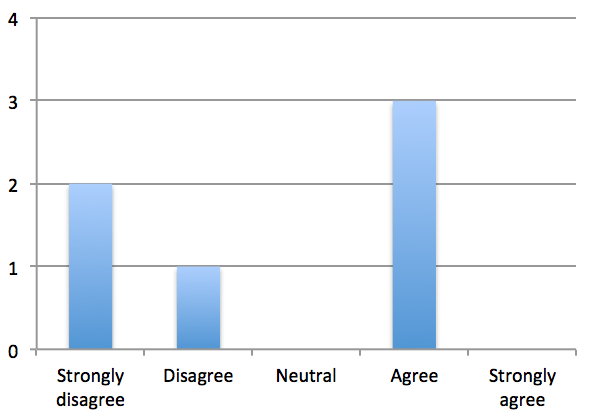
\includegraphics[width=1\linewidth]{./Images/graph1.png}%
          	}
          	\medskip
          	\centerline{Graph 1: Answers to question 1}
          \end{minipage}
\end{itemize}
\newpage
\begin{itemize}
		\item[] \textbf{Question 2:} I find the product unnecessarily complex
		\item[] \begin{minipage}[t]{\linewidth}
         	 \raggedright
          	\adjustbox{valign=t}{%
            		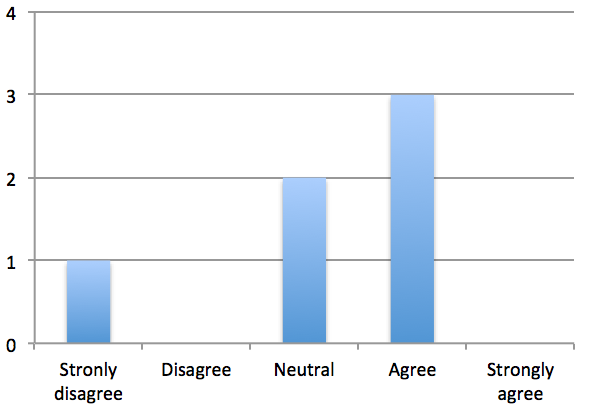
\includegraphics[width=1\linewidth]{./Images/graph2.png}%
          	}
          	\medskip
          	\centerline{Graph 2: Answers to question 2}
          \end{minipage}
\end{itemize}
\begin{itemize}
		\item[] \textbf{Question 3:} I find the product easy to use
		\item[] \begin{minipage}[t]{\linewidth}
         	 \raggedright
          	\adjustbox{valign=t}{%
            		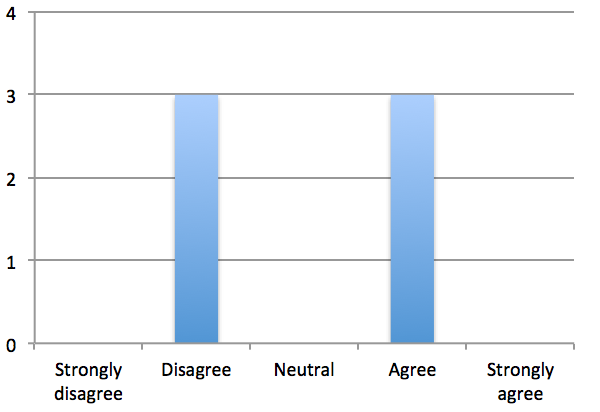
\includegraphics[width=1\linewidth]{./Images/graph3.png}%
          	}
          	\medskip
          	\centerline{Graph 3: Answers to question 3}
          \end{minipage}
\end{itemize}
\newpage
\begin{itemize}
		\item[] \textbf{Question 4:} I think I would need a technical person to use this product
		\item[] \begin{minipage}[t]{\linewidth}
         	 \raggedright
          	\adjustbox{valign=t}{%
            		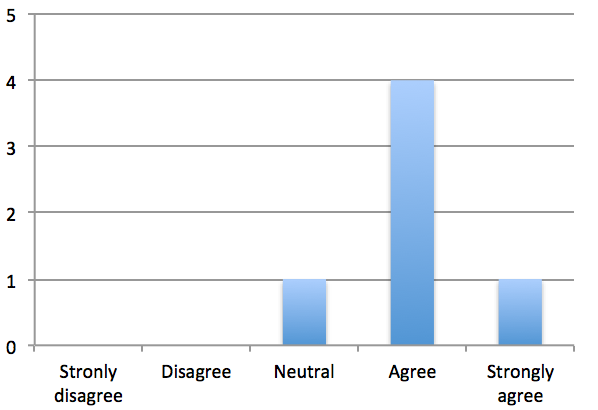
\includegraphics[width=1\linewidth]{./Images/graph4.png}%
          	}
          	\medskip
          	\centerline{Graph 4: Answers to question 4}
          \end{minipage}
\end{itemize}
\begin{itemize}
		\item[] \textbf{Question 5:} I find that the different functions of the product are clear
		\item[] \begin{minipage}[t]{\linewidth}
         	 \raggedright
          	\adjustbox{valign=t}{%
            		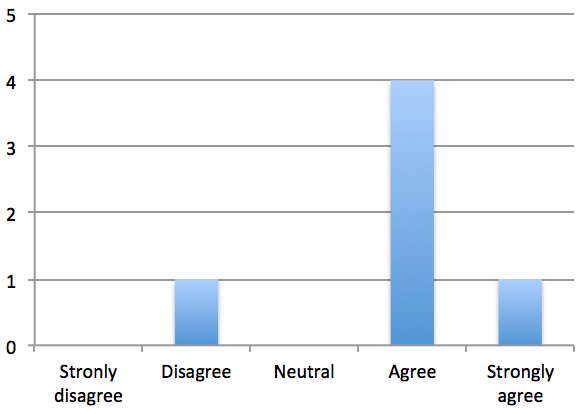
\includegraphics[width=1\linewidth]{./Images/graph5.png}%
          	}
          	\medskip
          	\centerline{Graph 5: Answers to question 5}
          \end{minipage}
\end{itemize}
\newpage
\begin{itemize}
		\item[] \textbf{Question 6:} I find the product inconsistent
		\item[] \begin{minipage}[t]{\linewidth}
         	 \raggedright
          	\adjustbox{valign=t}{%
            		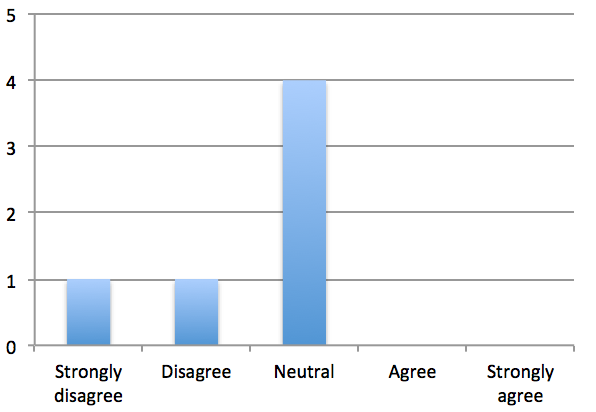
\includegraphics[width=1\linewidth]{./Images/graph6.png}%
          	}
          	\medskip
          	\centerline{Graph 6: Answers to question 6}
          \end{minipage}
\end{itemize}
\begin{itemize}
		\item[] \textbf{Question 7:} I think most people will easily learn to work with the product
		\item[] \begin{minipage}[t]{\linewidth}
         	 \raggedright
          	\adjustbox{valign=t}{%
            		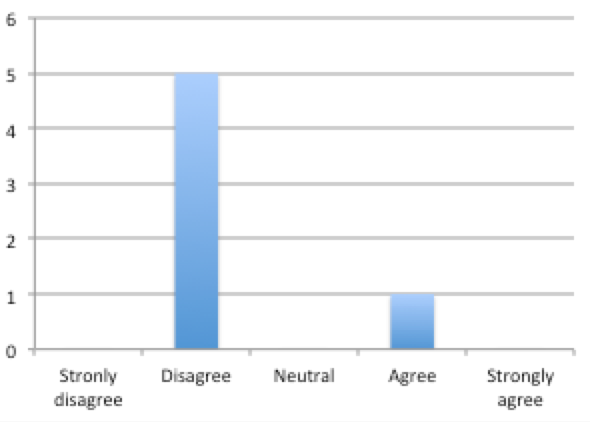
\includegraphics[width=1\linewidth]{./Images/graph7.png}%
          	}
          	\medskip
          	\centerline{Graph 7: Answers to question 7}
          \end{minipage}
\end{itemize}
\newpage
\begin{itemize}
		\item[] \textbf{Question 8:} I find the product awkward to work with
		\item[] \begin{minipage}[t]{\linewidth}
         	 \raggedright
          	\adjustbox{valign=t}{%
            		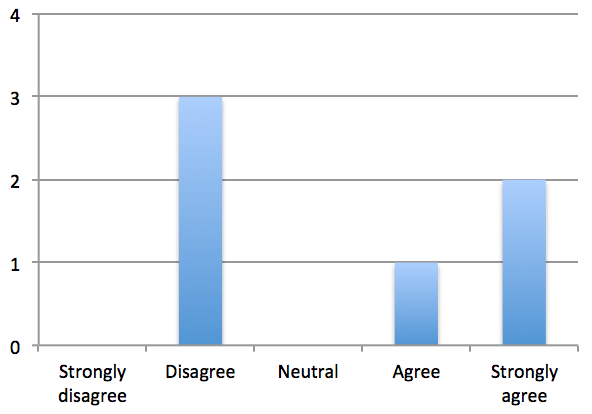
\includegraphics[width=1\linewidth]{./Images/graph8.png}%
          	}
          	\medskip
          	\centerline{Graph 8: Answers to question 8}
          \end{minipage}
\end{itemize}
\begin{itemize}
		\item[] \textbf{Question 9:} I find it easy to see what functions are available when using the product
		\item[] \begin{minipage}[t]{\linewidth}
         	 \raggedright
          	\adjustbox{valign=t}{%
            		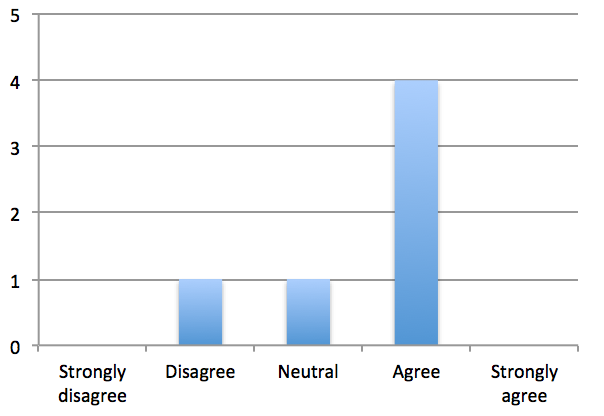
\includegraphics[width=1\linewidth]{./Images/graph9.png}%
          	}
          	\medskip
          	\centerline{Graph 9: Answers to question 9}
          \end{minipage}
\end{itemize}
\newpage
\begin{itemize}
		\item[] \textbf{Question 10:} I had to learn a lot before being able to use the product
		\item[] \begin{minipage}[t]{\linewidth}
         	 \raggedright
          	\adjustbox{valign=t}{%
            		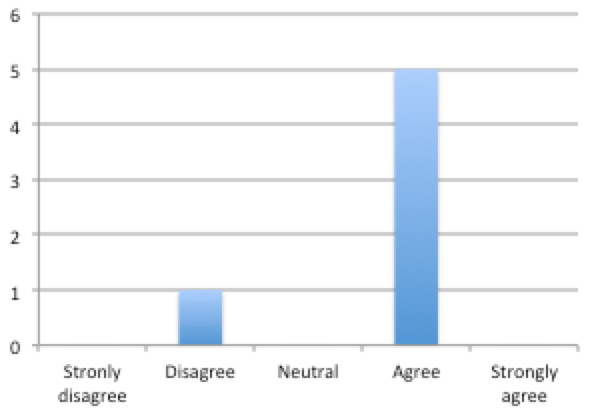
\includegraphics[width=1\linewidth]{./Images/graph10.png}%
          	}
          	\medskip
          	\centerline{Graph 10: Answers to question 10}
          \end{minipage}
\end{itemize}


\subsubsection{Explanation}

Once the design of the application was finished, we could start with a summative evaluation. We did this by using the observational evaluation technique talk aloud. We let six people, two parents and four friends, test our application by giving them several tasks and writing down how they used our application to achieve the goal of those tasks. An example task was to check the files that had a certain tag. We would then write down how the user navigated through the different screens. Another task was to try and create a group and then add atag to that group. Something noteworthy is that we asked the users to talk about what they are doing and if they were stuck, to tell us what they were searching for. The overall outcome of this evaluation was that our application is not ready for for real-world usage and that several improvements should be done before publishing the application. We will now discuss the answers to each question in more detail.

We see that the answers to the first question (I think I would use the product often) are very divergent. We think that this is because some people just really like the innovation that our project brings, but others might be used to the standard \texttt{WIMP}. When we asked for some feedback, we got two types of replies. The first type was that people didn't see the use of replacing the mouse with the Myo bracelet. This might be because using the Myo brings some overhead and it is also easy to get fatigue in your arm muscles by using it. The other type of reply was that they liked it because it was \textit{something different}, but not necessarily better.

"I find the product unnecessarily complex". With this question we wanted to know if the combination of different gestures and the concepts of groups and tags wouldn't be too complicated for regular users. The answers made clear that most of the evaluators indeed found that our application was too complex. These evaluators are all used to a regular filebrowser and don't necessarily find the concepts of groups and tags beneficial to use. Only one of our friends was fully supportive of our project and saw the possibilities that groups and tags bring.

The opinions were divided for the third question. This question basically tested the usability of our application. Some people seem to struggle when testing our project, while others don't seem to have any problems with it. We do have to note that for some users, the Myo bracelet was detecting less gestures than for other users. This might have impacted the results.

Question four goes hand in hand with the second question. It seems that most people agree on needing a technical person to use the application. This somewhat baffled us because we didn't expect the results to be so one-sided. A possible explanation is that we needed to help each evaluator with synchronizing the Myo. This required the evaluator to perform a gesture for some time and afterwards we also needed to calibrate the Myo to detect the bounds of our application.

Next to the complexity of our application, we also wanted to know what the user thought of our application flow. Although the fact that the evaluators found our application slightly too complex, they also found that the flow of the application was a good and logically structured flow. This wasn't that much of a surprise, since we are basically implementing the filesystem all over again, but with some conceptual and design changes.

When asking if people found our application inconsistent, most of the evaluators didn't really have an opinion. This might be because they didn't fully understand the question. What we wanted to know, was that when a user wants to perform some task, he has to perform a sequence of actions. If he then wants to perform a similar task, he should also perform a similar action sequence. The evaluators who did understand the question, all answered that our application is consistent.

The overall outcome of question seven is that our application would be hard to learn. Although we don't agree on this, we do understand why people might think in this way. When we asked these people to evaluate our application, they all had to learn the gestures and functionalities in a limited time frame. This probably influenced them in a negative manner, resulting in these answers.

"I find the product awkward to work with". This question was based on the fact that people do have to make strange gestures in front of their screen, which might be a bit awkward. With awkward, me meant that the user might feel uncomfortable when using the application, but also that the user did not find it handy to use the Myo bracelet. 50\% of the evaluators were uncomfortable when using the application. This is a rather high percentage, which might indicate that the world isn't ready to combine working on a computer and using gestures to control that computer.

We attempted to display as much relevant information as possible on the screen, which resulted in a positive evaluation for question nine. Users seem to know what the enabled tasks are when they use our application. We are very happy that this is the case, since using a file browser should be intuitive and should not take that much time to perform a certain task.

Question ten is very similar to question seven. We again suspect that the limited time frame to learn and understand the different gestures and functionalities might have influenced the different evaluators. We could argue that these answers might be a bit too subjective. When they first introduced a mouse as a pointer, people also had to learn how to use it and what the different mouse buttons did.

\section{Conclusion}
To conclude, we think that our application is not ready for real-world usage. The project was interesting to develop, however the usability is limited. This is mainly because of the Myo and missing functionalities in our application due to the limited time. We think that, after a few years of development of the Myo, there will be a more accurate detection of gestures and possibly a way to define our own gestures. The five gestures that are currently available are too limited to interact with the screen and to map functionalities to specific gestures. Nevertheless, we expect that in the future gesture-based interaction will become more popular then mouse-based interaction.

\end{document}
